\section{Comparando soluciones}
Para comparar las la calidad de las distintas soluciones, además del valor objetivo se compara con 
la cantidad de elementos iguales en toda la solución y la cantidad igual de elementos para cada 
bundle. De esta manera se observa que tan \textquotedblleft parecidas\textquotedblright son las 
soluciones y con más detalle que tan \textquotedblleft parecidos\textquotedblright son los bundles. 
Entre los diferentes algoritmos buscamos la cantidad de elementos iguales en cada una de las 
soluciones y también la cantidad de elementos iguales por bundle.
\section{Papers}
Originalmente la base de datos contenía unos 7777 papers, de los cuáles se tuvo que hacer una 
depuración, ya que había papers que no tenían ningún autor asociado o perfil creado. Luego de la 
depuración obtuvimos 4937 que cumplen los requisitos para la búsqueda de las soluciones.\\
Se genraron soluciones con las siguientes características:\\
\Solucion
{}
{simple, por tuplas y proporcional}
{\texttt{HAC} y \texttt{BOBO-x}, con  $x \in$ $(10, 160)$}
{$\in$ $(0,1; 0,3; 0,5; 0,7; 0,9)$}
{10}
{5}
Como primera observación podemos ver la cantidad de bundles que se generan para cada algoritmo de 
producción:\\
\begin{table}[h]
  \centering
  \resizebox{\textwidth}{!} {
    \begin{tabular}{|lcc|}
    \hline
    Algoritmo & Bundles Generados & Tiempo de Ejecución (minutos) \\
    \hline
    HAC       & $2378$ & $6$ \\
    BOBO-10   & $100$  & $2$ \\
    BOBO-160  & $1600$ & $5$ \\
    \hline
    \end{tabular}
  }
    \caption {Cantidad de bundles generados antes de la selección final}
\end{table}

En los siguientes gráficos se visualiza los resultados obtenidos para los gammas 0.1 y 0.9. Cada 
nodo representa un bundle y los ejes el valor de la similitud entre cada uno de ellos. La línea más 
gruesa indica un mayor grado de similitud. En cuanto a los vértices al acercarse al azul el valor 
de la intra es menor y al rojo mayor.
\begin{figure}[H]
  \centering
    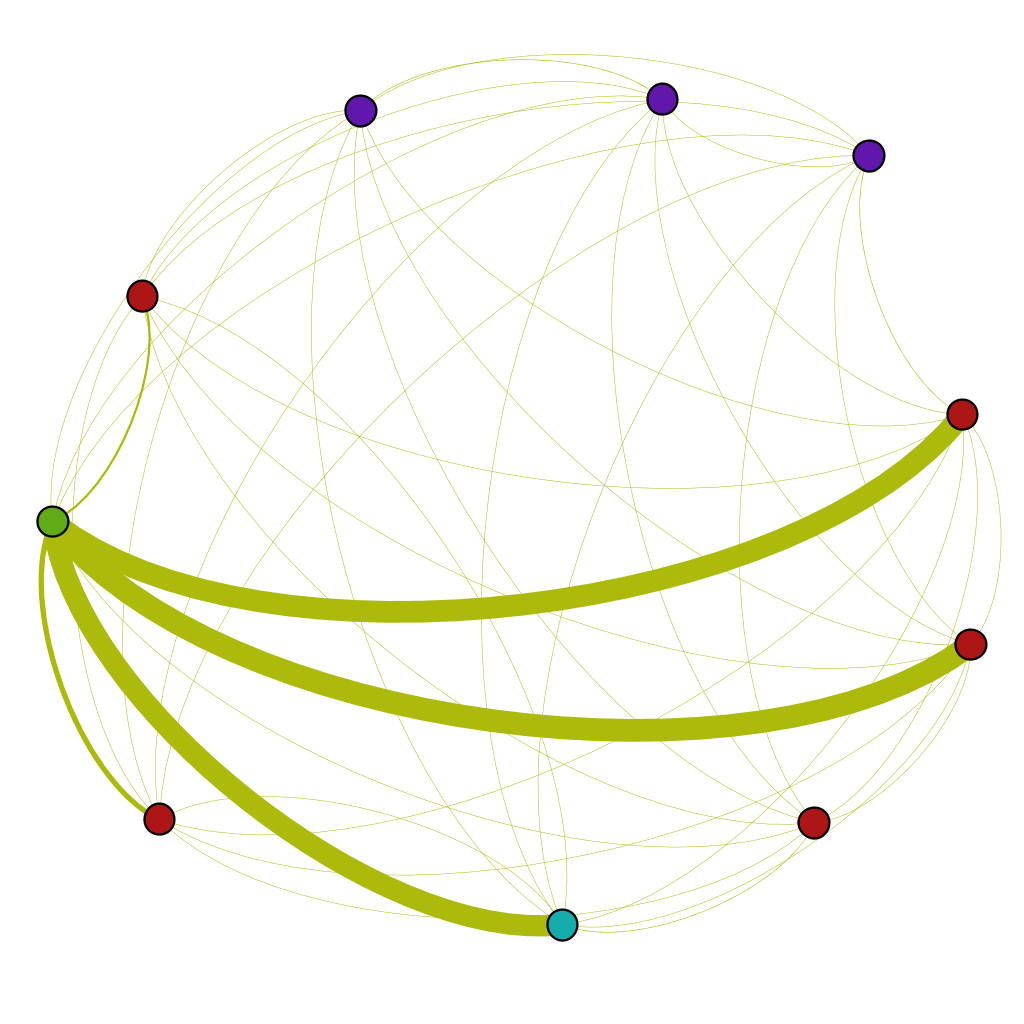
\includegraphics[width=0.5\textwidth]{resultados/papers/intra_inter/hac01.png}
  \caption{Relación entre bundles para $\gamma$ = $0.1$ y algoritmo HAC}
  \label{res:img-gamma01-hac}
\end{figure}

\begin{figure}[H]
  \centering
    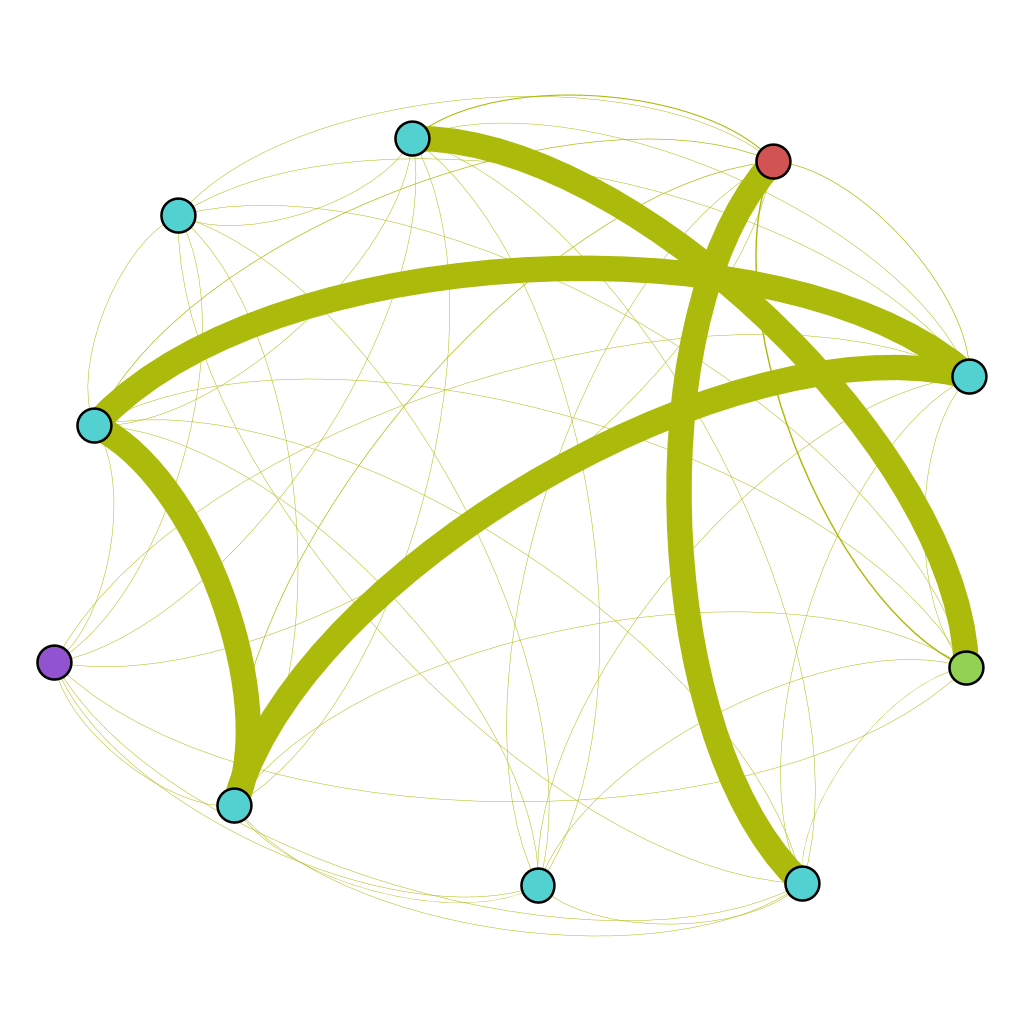
\includegraphics[width=0.5\textwidth]{resultados/papers/intra_inter/hac09.png}
  \caption{Relación entre bundles para $\gamma$ = $0.9$ y algoritmo HAC}
  \label{res:img-gamma09-hac}
\end{figure}

\section{Autores}
Se genraron soluciones con las siguientes características:\\
\Solucion
{}
{simple y proporcional}
{\texttt{HAC} y \texttt{BOBO-x}, con  $x \in$ $(10, 160)$ y \texttt{BOBO-ex}}
{$\in$ $(0,1; 0,3; 0,5; 0,7; 0,9)$}
{10 y 20}
{5 y 10}

Para todas las soluciones obtenidas con la generación \texttt{HAC} y utilizando cualquiera de los 
dos algoritmos de selección de selección, todas las soluciones formaron los mismos bundles a 
pesar de que el $\gamma$ sea distinto.\\ 
Se realizaron otras búsquedas de soluciones, excluyendo a cinco de los autores que están presentes 
en todas las soluciones. En las nuevas soluciones obtenidas se repite nuevamente el comportamiento 
que para todos los $\gamma$, con las soluciones idénticas y valores de la función objetivo coinciden 
con los de las soluciones obtenidas sin excluir autores.\\
Con el algoritmo \texttt{HAC} todas las soluciones fueron idénticas para todos los $\gamma$. Esto 
se debe a que existen $40000$ relaciones de similitud con valor uno. Con la heurística Produce and 
Choose, al momento de producir no se tiene en cuenta el $\gamma$ por lo tanto para todos los 
$\gamma$ en la etapa de producción se producen los mismos bundles.\\
Por otro lado todas las soluciones generadas por el algoritmo \texttt{HAC} prácticamente no 
comparten bundles similares con las demás soluciones, ni siquiera autores similares en toda la 
solución.

\section{Búsqueda con perfil específico}
En una primera aproximación para realizar esta búsqueda solo se modifico la generación de bundles, 
lo cuál, si bien genero resultados diferentes al algoritmo original, no se veía reflejado en los 
resultados las temáticas de los bundles con la elegida para la búsqueda. \\
A partir de ello se decidió modificar también la selección de los bundles para intentar obtener 
bundles relevantes con el perfil elegido. \\
A continuación mostramos la temáticas obtenidas para una búsqueda con un perfil específico de 
ALGORITHM = 50 \%, DISTRIBUTED SYSTEMS = 25 \% y KNOWLEDGE ENGINEERING = 25 \% para la ejecución 
del algoritmo jerárquico con $\gamma$ = 0.1 y $\gamma$ = 0.9.
\begin{figure}
  \centering
    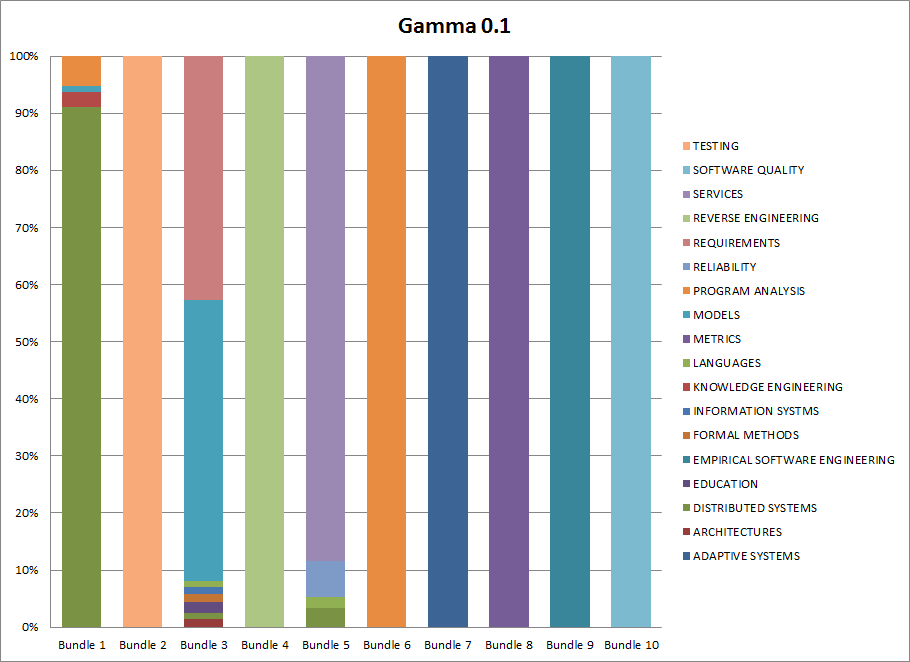
\includegraphics[width=\textwidth]{resultados/papers/intra_inter/grafico_gamm01.png}
  \caption{$\gamma$ = 0.1}
  \label{res:img-gamma01-especifico}
\end{figure}

\begin{figure}
  \centering
    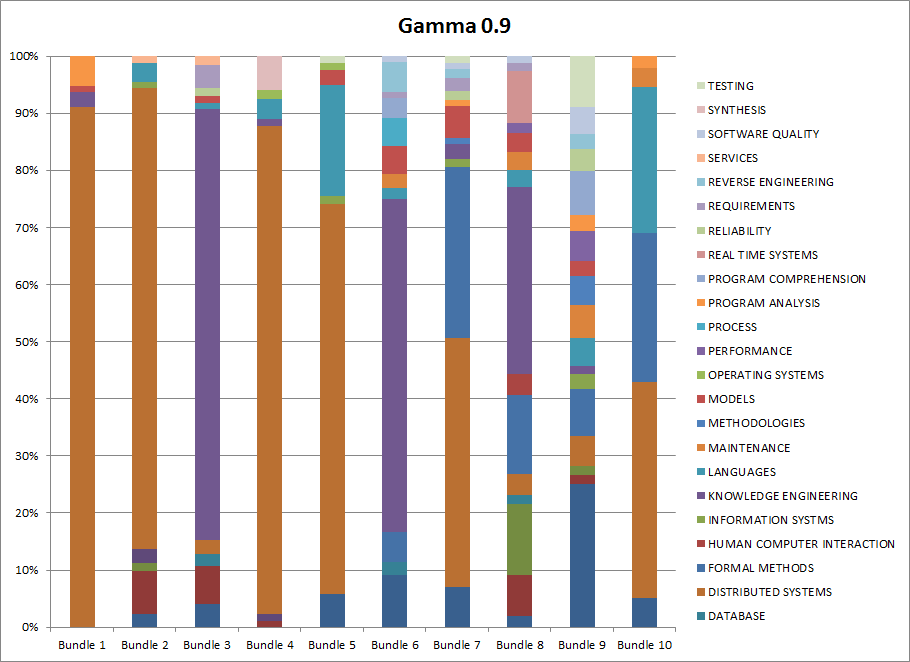
\includegraphics[width=\textwidth]{resultados/papers/intra_inter/grafico_gamm09.png}
  \caption{$\gamma$ = 0.9}
  \label{res:img-gamma09-especifico}
\end{figure}